\documentclass{extbook}[14pt]
\usepackage{multicol, enumerate, enumitem, hyperref, color, soul, setspace, parskip, fancyhdr, amssymb, amsthm, amsmath, latexsym, units, mathtools}
\everymath{\displaystyle}
\usepackage[headsep=0.5cm,headheight=0cm, left=1 in,right= 1 in,top= 1 in,bottom= 1 in]{geometry}
\usepackage{dashrule}  % Package to use the command below to create lines between items
\newcommand{\litem}[1]{\item #1

\rule{\textwidth}{0.4pt}}
\pagestyle{fancy}
\lhead{}
\chead{Answer Key for Progress Quiz 6 Version B}
\rhead{}
\lfoot{1430-1829}
\cfoot{}
\rfoot{test}
\begin{document}
\textbf{This key should allow you to understand why you choose the option you did (beyond just getting a question right or wrong). \href{https://xronos.clas.ufl.edu/mac1105spring2020/courseDescriptionAndMisc/Exams/LearningFromResults}{More instructions on how to use this key can be found here}.}

\textbf{If you have a suggestion to make the keys better, \href{https://forms.gle/CZkbZmPbC9XALEE88}{please fill out the short survey here}.}

\textit{Note: This key is auto-generated and may contain issues and/or errors. The keys are reviewed after each exam to ensure grading is done accurately. If there are issues (like duplicate options), they are noted in the offline gradebook. The keys are a work-in-progress to give students as many resources to improve as possible.}

\rule{\textwidth}{0.4pt}

\begin{enumerate}\litem{
Construct the lowest-degree polynomial given the zeros below. Then, choose the intervals that contain the coefficients of the polynomial in the form $x^3+bx^2+cx+d$.
\[ -4 - 5 i \text{ and } 1 \]The solution is \( x^{3} +7 x^{2} +33 x -41 \), which is option D.\begin{enumerate}[label=\Alph*.]
\item \( b \in [-3, 2], c \in [3.3, 7.3], \text{ and } d \in [-5.77, -4.52] \)

$x^{3} + x^{2} +4 x -5$, which corresponds to multiplying out $(x + 5)(x -1)$.
\item \( b \in [-19, -6], c \in [32, 33.7], \text{ and } d \in [39.4, 41.41] \)

$x^{3} -7 x^{2} +33 x + 41$, which corresponds to multiplying out $(x-(-4 - 5 i))(x-(-4 + 5 i))(x + 1)$.
\item \( b \in [-3, 2], c \in [-1, 3.5], \text{ and } d \in [-4.47, -3.55] \)

$x^{3} + x^{2} +3 x -4$, which corresponds to multiplying out $(x + 4)(x -1)$.
\item \( b \in [2, 9], c \in [32, 33.7], \text{ and } d \in [-41.76, -39.64] \)

* $x^{3} +7 x^{2} +33 x -41$, which is the correct option.
\item \( \text{None of the above.} \)

This corresponds to making an unanticipated error or not understanding how to use nonreal complex numbers to create the lowest-degree polynomial. If you chose this and are not sure what you did wrong, please contact the coordinator for help.
\end{enumerate}

\textbf{General Comment:} Remember that the conjugate of $a+bi$ is $a-bi$. Since these zeros always come in pairs, we need to multiply out $(x-(-4 - 5 i))(x-(-4 + 5 i))(x-(1))$.
}
\litem{
Describe the end behavior of the polynomial below.
\[ f(x) = 2(x + 9)^{2}(x - 9)^{5}(x + 6)^{3}(x - 6)^{4} \]The solution is the graph below, which is option C.
\begin{center}
    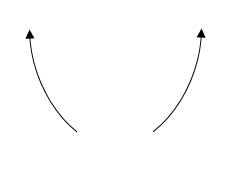
\includegraphics[width=0.3\textwidth]{../Figures/polyEndBehaviorCopyCB.png}
\end{center}\begin{enumerate}[label=\Alph*.]
\begin{multicols}{2}
\item 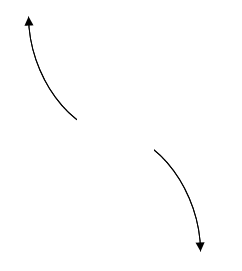
\includegraphics[width = 0.3\textwidth]{../Figures/polyEndBehaviorCopyAB.png}
\item 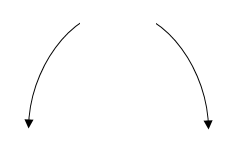
\includegraphics[width = 0.3\textwidth]{../Figures/polyEndBehaviorCopyBB.png}
\item 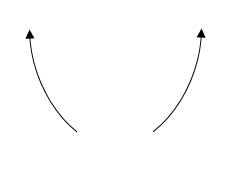
\includegraphics[width = 0.3\textwidth]{../Figures/polyEndBehaviorCopyCB.png}
\item 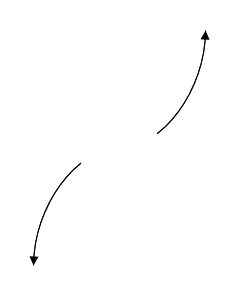
\includegraphics[width = 0.3\textwidth]{../Figures/polyEndBehaviorCopyDB.png}
\end{multicols}\item None of the above.\end{enumerate}
\textbf{General Comment:} Remember that end behavior is determined by the leading coefficient AND whether the \textbf{sum} of the multiplicities is positive or negative.
}
\litem{
Describe the zero behavior of the zero $x = 5$ of the polynomial below.
\[ f(x) = -6(x + 7)^{10}(x - 7)^{8}(x + 5)^{12}(x - 5)^{9} \]The solution is the graph below, which is option A.
\begin{center}
    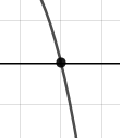
\includegraphics[width=0.3\textwidth]{../Figures/polyZeroBehaviorAB.png}
\end{center}\begin{enumerate}[label=\Alph*.]
\begin{multicols}{2}
\item 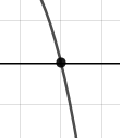
\includegraphics[width = 0.3\textwidth]{../Figures/polyZeroBehaviorAB.png}
\item 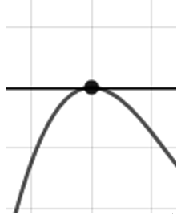
\includegraphics[width = 0.3\textwidth]{../Figures/polyZeroBehaviorBB.png}
\item 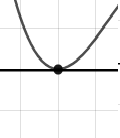
\includegraphics[width = 0.3\textwidth]{../Figures/polyZeroBehaviorCB.png}
\item 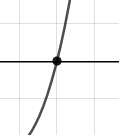
\includegraphics[width = 0.3\textwidth]{../Figures/polyZeroBehaviorDB.png}
\end{multicols}\item None of the above.\end{enumerate}
\textbf{General Comment:} You will need to sketch the entire graph, then zoom in on the zero the question asks about.
}
\litem{
Construct the lowest-degree polynomial given the zeros below. Then, choose the intervals that contain the coefficients of the polynomial in the form $ax^3+bx^2+cx+d$.
\[ \frac{-7}{5}, -4, \text{ and } \frac{-6}{5} \]The solution is \( 25x^{3} +165 x^{2} +302 x + 168 \), which is option A.\begin{enumerate}[label=\Alph*.]
\item \( a \in [24, 27], b \in [159, 167], c \in [296, 309], \text{ and } d \in [166, 170] \)

* $25x^{3} +165 x^{2} +302 x + 168$, which is the correct option.
\item \( a \in [24, 27], b \in [159, 167], c \in [296, 309], \text{ and } d \in [-168, -161] \)

$25x^{3} +165 x^{2} +302 x -168$, which corresponds to multiplying everything correctly except the constant term.
\item \( a \in [24, 27], b \in [-109, -104], c \in [-28, -20], \text{ and } d \in [166, 170] \)

$25x^{3} -105 x^{2} -22 x + 168$, which corresponds to multiplying out $(5x -7)(x -4)(5x + 6)$.
\item \( a \in [24, 27], b \in [90, 102], c \in [-63, -56], \text{ and } d \in [-168, -161] \)

$25x^{3} +95 x^{2} -62 x -168$, which corresponds to multiplying out $(5x -7)(x + 4)(5x + 6)$.
\item \( a \in [24, 27], b \in [-166, -163], c \in [296, 309], \text{ and } d \in [-168, -161] \)

$25x^{3} -165 x^{2} +302 x -168$, which corresponds to multiplying out $(5x -7)(x -4)(5x -6)$.
\end{enumerate}

\textbf{General Comment:} To construct the lowest-degree polynomial, you want to multiply out $(5x + 7)(x + 4)(5x + 6)$
}
\litem{
Construct the lowest-degree polynomial given the zeros below. Then, choose the intervals that contain the coefficients of the polynomial in the form $ax^3+bx^2+cx+d$.
\[ \frac{5}{2}, \frac{-7}{5}, \text{ and } -5 \]The solution is \( 10x^{3} +39 x^{2} -90 x -175 \), which is option D.\begin{enumerate}[label=\Alph*.]
\item \( a \in [9, 12], b \in [38, 45], c \in [-91, -85], \text{ and } d \in [171, 181] \)

$10x^{3} +39 x^{2} -90 x + 175$, which corresponds to multiplying everything correctly except the constant term.
\item \( a \in [9, 12], b \in [-45, -32], c \in [-91, -85], \text{ and } d \in [171, 181] \)

$10x^{3} -39 x^{2} -90 x + 175$, which corresponds to multiplying out $(2x + 5)(5x -7)(x -5)$.
\item \( a \in [9, 12], b \in [55, 66], c \in [17, 22], \text{ and } d \in [-178, -168] \)

$10x^{3} +61 x^{2} +20 x -175$, which corresponds to multiplying out $(2x + 5)(5x -7)(x + 5)$.
\item \( a \in [9, 12], b \in [38, 45], c \in [-91, -85], \text{ and } d \in [-178, -168] \)

* $10x^{3} +39 x^{2} -90 x -175$, which is the correct option.
\item \( a \in [9, 12], b \in [83, 95], c \in [227, 235], \text{ and } d \in [171, 181] \)

$10x^{3} +89 x^{2} +230 x + 175$, which corresponds to multiplying out $(2x + 5)(5x + 7)(x + 5)$.
\end{enumerate}

\textbf{General Comment:} To construct the lowest-degree polynomial, you want to multiply out $(2x -5)(5x + 7)(x + 5)$
}
\litem{
Which of the following equations \textit{could} be of the graph presented below?

\begin{center}
    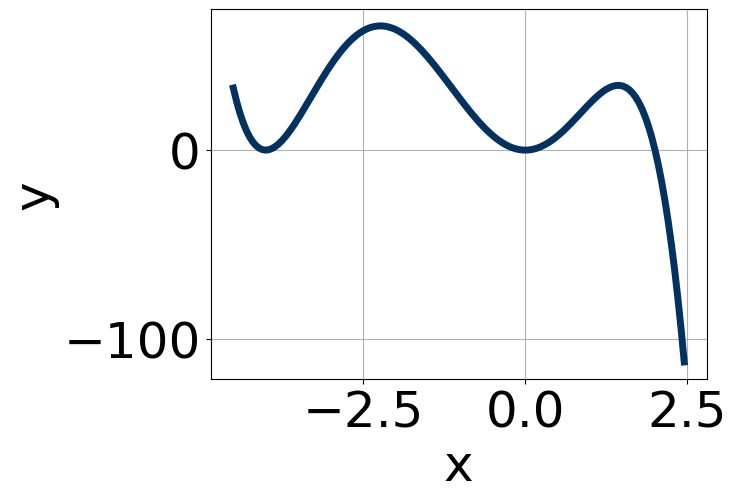
\includegraphics[width=0.5\textwidth]{../Figures/polyGraphToFunctionCopyB.png}
\end{center}


The solution is \( -2x^{4} (x - 2)^{8} (x + 1)^{4} \), which is option A.\begin{enumerate}[label=\Alph*.]
\item \( -2x^{4} (x - 2)^{8} (x + 1)^{4} \)

* This is the correct option.
\item \( 17x^{6} (x - 2)^{4} (x + 1)^{9} \)

The factor $(x + 1)$ should have an even power and the leading coefficient should be the opposite sign.
\item \( -12x^{9} (x - 2)^{10} (x + 1)^{7} \)

The factors $x$ and $(x + 1)$ should both have even powers.
\item \( -17x^{4} (x - 2)^{6} (x + 1)^{9} \)

The factor $(x + 1)$ should have an even power.
\item \( 11x^{6} (x - 2)^{4} (x + 1)^{8} \)

This corresponds to the leading coefficient being the opposite value than it should be.
\end{enumerate}

\textbf{General Comment:} General Comments: Draw the x-axis to determine which zeros are touching (and so have even multiplicity) or cross (and have odd multiplicity).
}
\litem{
Which of the following equations \textit{could} be of the graph presented below?

\begin{center}
    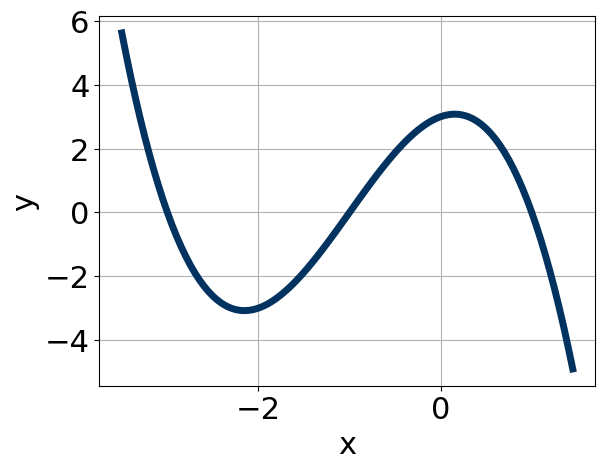
\includegraphics[width=0.5\textwidth]{../Figures/polyGraphToFunctionB.png}
\end{center}


The solution is \( -16x^{11} (x + 3)^{4} (x + 4)^{4} \), which is option A.\begin{enumerate}[label=\Alph*.]
\item \( -16x^{11} (x + 3)^{4} (x + 4)^{4} \)

* This is the correct option.
\item \( -10x^{10} (x + 3)^{10} (x + 4)^{11} \)

The factor $(x + 4)$ should have an even power and the factor $x$ should have an odd power.
\item \( 10x^{9} (x + 3)^{8} (x + 4)^{4} \)

This corresponds to the leading coefficient being the opposite value than it should be.
\item \( 18x^{6} (x + 3)^{6} (x + 4)^{10} \)

The factor $x$ should have an odd power and the leading coefficient should be the opposite sign.
\item \( -15x^{11} (x + 3)^{8} (x + 4)^{9} \)

The factor $(x + 4)$ should have an even power.
\end{enumerate}

\textbf{General Comment:} General Comments: Draw the x-axis to determine which zeros are touching (and so have even multiplicity) or cross (and have odd multiplicity).
}
\litem{
Describe the zero behavior of the zero $x = -2$ of the polynomial below.
\[ f(x) = 9(x + 2)^{9}(x - 2)^{14}(x + 7)^{4}(x - 7)^{8} \]The solution is the graph below, which is option D.
\begin{center}
    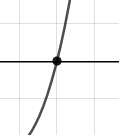
\includegraphics[width=0.3\textwidth]{../Figures/polyZeroBehaviorCopyDB.png}
\end{center}\begin{enumerate}[label=\Alph*.]
\begin{multicols}{2}
\item 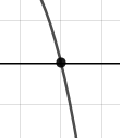
\includegraphics[width = 0.3\textwidth]{../Figures/polyZeroBehaviorCopyAB.png}
\item 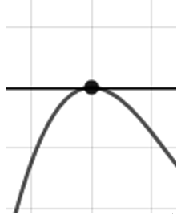
\includegraphics[width = 0.3\textwidth]{../Figures/polyZeroBehaviorCopyBB.png}
\item 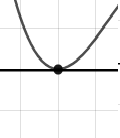
\includegraphics[width = 0.3\textwidth]{../Figures/polyZeroBehaviorCopyCB.png}
\item 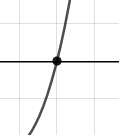
\includegraphics[width = 0.3\textwidth]{../Figures/polyZeroBehaviorCopyDB.png}
\end{multicols}\item None of the above.\end{enumerate}
\textbf{General Comment:} You will need to sketch the entire graph, then zoom in on the zero the question asks about.
}
\litem{
Construct the lowest-degree polynomial given the zeros below. Then, choose the intervals that contain the coefficients of the polynomial in the form $x^3+bx^2+cx+d$.
\[ 4 + 2 i \text{ and } 3 \]The solution is \( x^{3} -11 x^{2} +44 x -60 \), which is option B.\begin{enumerate}[label=\Alph*.]
\item \( b \in [-3, 2], c \in [-8.19, -6.43], \text{ and } d \in [12, 18] \)

$x^{3} + x^{2} -7 x + 12$, which corresponds to multiplying out $(x -4)(x -3)$.
\item \( b \in [-18, -8], c \in [42.96, 45.21], \text{ and } d \in [-60, -55] \)

* $x^{3} -11 x^{2} +44 x -60$, which is the correct option.
\item \( b \in [10, 12], c \in [42.96, 45.21], \text{ and } d \in [53, 64] \)

$x^{3} +11 x^{2} +44 x + 60$, which corresponds to multiplying out $(x-(4 + 2 i))(x-(4 - 2 i))(x + 3)$.
\item \( b \in [-3, 2], c \in [-5.57, -3.76], \text{ and } d \in [-2, 10] \)

$x^{3} + x^{2} -5 x + 6$, which corresponds to multiplying out $(x -2)(x -3)$.
\item \( \text{None of the above.} \)

This corresponds to making an unanticipated error or not understanding how to use nonreal complex numbers to create the lowest-degree polynomial. If you chose this and are not sure what you did wrong, please contact the coordinator for help.
\end{enumerate}

\textbf{General Comment:} Remember that the conjugate of $a+bi$ is $a-bi$. Since these zeros always come in pairs, we need to multiply out $(x-(4 + 2 i))(x-(4 - 2 i))(x-(3))$.
}
\litem{
Describe the end behavior of the polynomial below.
\[ f(x) = -4(x + 4)^{5}(x - 4)^{6}(x - 5)^{2}(x + 5)^{2} \]The solution is the graph below, which is option A.
\begin{center}
    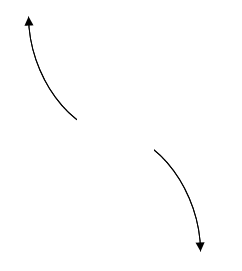
\includegraphics[width=0.3\textwidth]{../Figures/polyEndBehaviorAB.png}
\end{center}\begin{enumerate}[label=\Alph*.]
\begin{multicols}{2}
\item 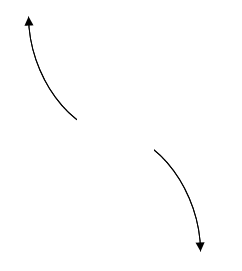
\includegraphics[width = 0.3\textwidth]{../Figures/polyEndBehaviorAB.png}
\item 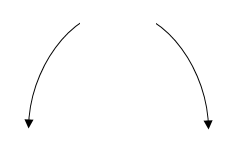
\includegraphics[width = 0.3\textwidth]{../Figures/polyEndBehaviorBB.png}
\item 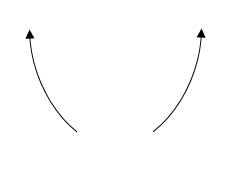
\includegraphics[width = 0.3\textwidth]{../Figures/polyEndBehaviorCB.png}
\item 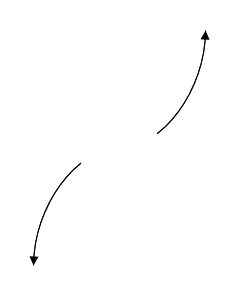
\includegraphics[width = 0.3\textwidth]{../Figures/polyEndBehaviorDB.png}
\end{multicols}\item None of the above.\end{enumerate}
\textbf{General Comment:} Remember that end behavior is determined by the leading coefficient AND whether the \textbf{sum} of the multiplicities is positive or negative.
}
\end{enumerate}

\end{document}